% Gerado de docs/monografia/03-sistema.md por scripts/monografia_latex.py.
% Não edite aqui: edite o .md e gere de novo.

\chapter{\texorpdfstring{\mbox{O} \mbox{SISTEMA} \mbox{STRUCTURA}}{O SISTEMA STRUCTURA}}\label{cap:3}

Este capítulo descreve o sistema na versão de 19/11/2026: o domínio que ele ensina (3.1); a forma como diagnostica cada estudante (3.2); o percurso que oferece a partir do diagnóstico (3.3); as três peças de conteúdo que sustentam esse percurso, que são a escada de passos (3.4), a demonstração com previsão (3.5) e a cena que anima a revisão de cada premissa (3.6); o registro da sessão (3.7); e a interface (3.8). A arquitetura de software está resumida em 3.9.

\section{O domínio: premissas, concepções errôneas e questões}

O conteúdo de ponteiros em C está organizado em 13 tópicos, da declaração de variáveis ao ponteiro pendente por escopo (Quadro~\ref{qua:3-1}). Cada tópico é um pequeno grafo de premissas: proposições curtas que o estudante pode afirmar ou negar. As premissas de base são fatos que se verificam olhando um programa (``\texttt{int notas[3]} cria três caixas de int grudadas''); as de inferência decorrem de outras, que são o seu suporte (``então \texttt{notas[i]} é só outro jeito de escrever \texttt{*(notas + i)}''). Os 13 tópicos somam 79 premissas, e a ordem de cada tópico respeita o suporte: nenhuma premissa vem antes de uma premissa que a sustenta.

\begin{quadro}[htbp]
\caption{Os tópicos}\label{qua:3-1}
\footnotesize
\begin{tabularx}{\textwidth}{|>{\centering\arraybackslash}p{1.7cm}|X|>{\centering\arraybackslash}p{2.4cm}|}
\hline
\textbf{Tópico} & \textbf{Título} & \textbf{Premissas} \\ \hline
kc\_00 & Declaração de variáveis & 5 \\ \hline
kc\_01 & Modelo de memória & 5 \\ \hline
kc\_02 & O que é um ponteiro & 6 \\ \hline
kc\_03 & Declaração e inicialização & 6 \\ \hline
kc\_04 & Dereferência: \& e * & 6 \\ \hline
kc\_05 & Ponteiro NULL & 6 \\ \hline
kc\_06 & Passagem por referência & 6 \\ \hline
kc\_07 & Ponteiro e array & 7 \\ \hline
kc\_08 & Alocação dinâmica & 6 \\ \hline
kc\_09 & free() e ponteiro pendente & 8 \\ \hline
kc\_10 & Ponteiro para ponteiro & 6 \\ \hline
kc\_11 & Aritmética de ponteiros & 6 \\ \hline
kc\_12 & Ponteiro pendente por escopo & 6 \\ \hline
\end{tabularx}
\fonte{Elaborado pelo autor.}
\end{quadro}

Cada concepção errônea do catálogo nega exatamente uma premissa. É o que transforma ``o estudante tem uma ideia errada'' num endereço: a crença de que ``o ponteiro é o próprio dado: retornar o endereço de uma local devolve a variável'' nega a premissa do kc\_12 segundo a qual retornar \texttt{\&local} copia o endereço, e não a caixa. O catálogo tem 61 concepções, cada uma com procedência declarada; o Capítulo 4 trata dessa procedência.

O banco de questões tem 560 questões de múltipla escolha, distribuídas pelas premissas, cada uma com um nível (do mais mecânico ao mais conceitual) e um uso (entrada, diagnóstico ou treino). Toda alternativa errada aponta a concepção errônea que a explicaria. É dessa ligação que o diagnóstico tira a razão de cada resposta.

Cada premissa tem ainda uma explicação curta, com a premissa em linguagem simples e um exemplo em código animado pela cena da premissa (3.6), que a pessoa pode abrir a qualquer momento pelo botão ``Ver a explicação''.

\section{O diagnóstico: resposta, razão e certeza}

Cada premissa começa por uma pergunta de diagnóstico, numa tela só (Figura~\ref{fig:3-1}). A pessoa marca a resposta, que pode trocar à vontade, e a confirma. Só então aparecem as razões possíveis (a certa é a premissa em linguagem simples, e as erradas são as concepções errôneas que as alternativas daquela questão apontam), e a resposta trava; por último vem a certeza: ``chutei'', ``acho que sei'' ou ``tenho certeza''. A ordem é deliberada. As razões dão pista de qual resposta combina com cada uma, e quem pudesse voltar depois de lê-las trocaria a resposta para combinar com a razão: o diagnóstico passaria a medir a leitura das razões, e não a ideia com que a pessoa respondeu. A confirmação antes das razões deixa corrigir um toque errado enquanto a resposta ainda não travou. Há também o botão ``Não sei'', que é uma resposta legítima: obrigar a escolher fabricaria chute, e com ele a lacuna vira dado observado, e não inferido.

\begin{figure}[htbp]
\centering
\caption{A pergunta de diagnóstico, com a resposta confirmada e as razões (kc\_07, tema claro)}\label{fig:3-1}
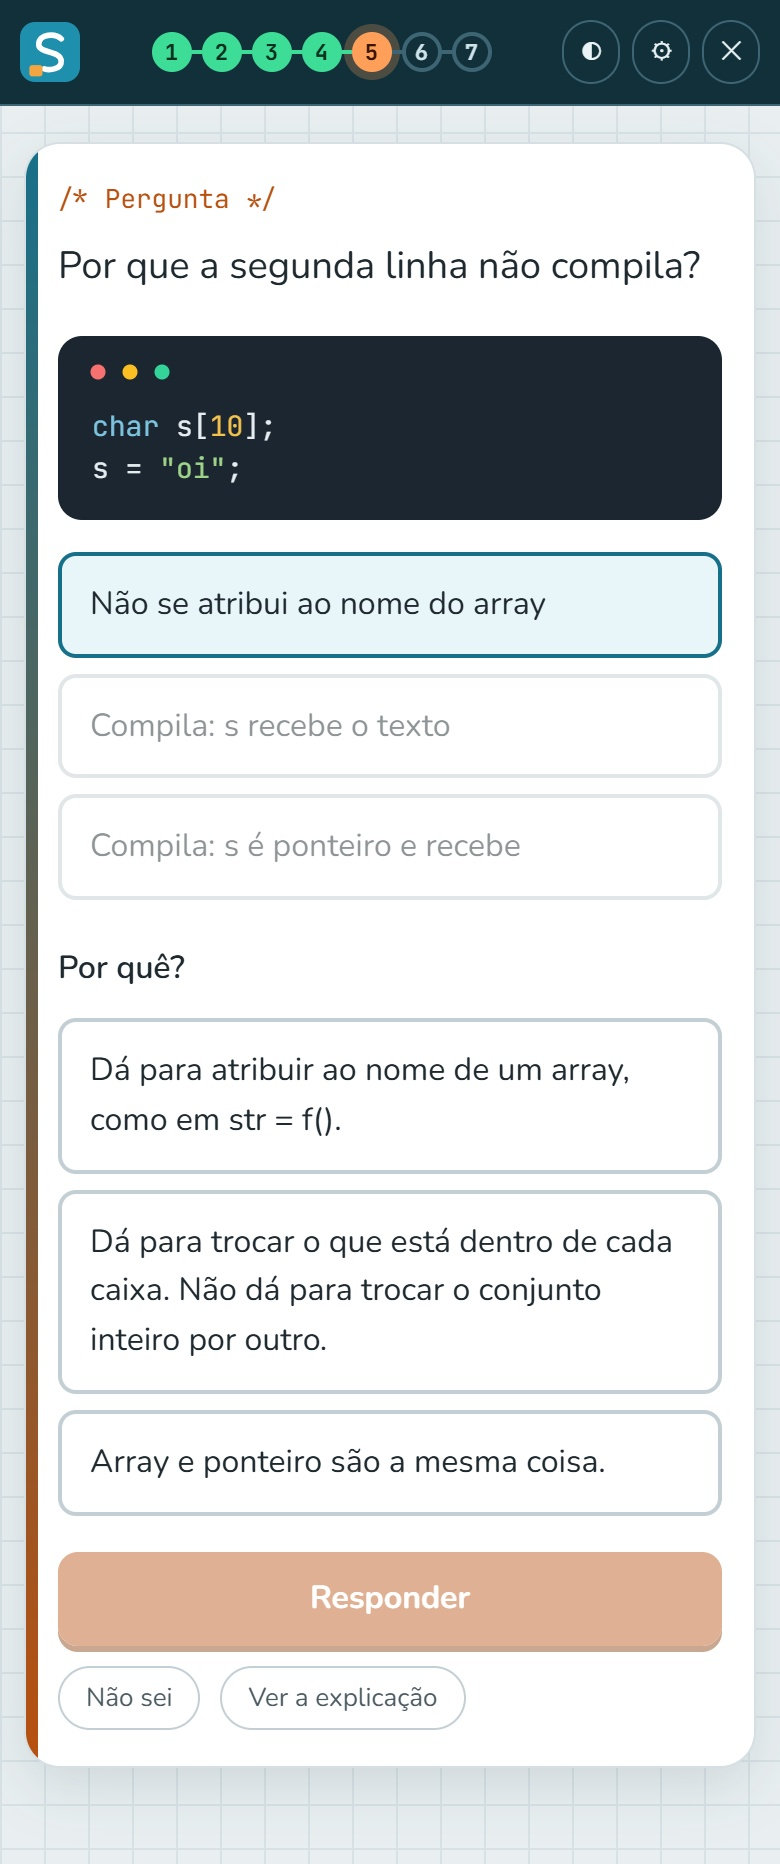
\includegraphics[width=.5\textwidth,height=.55\textheight,keepaspectratio]{fig-3-1-pergunta.jpg}
\fonte{Captura de tela do Structura, elaborada pelo autor.}
\end{figure}

A pergunta de abertura de cada premissa é, de preferência, uma questão com código de nível intermediário: a que pede que a pessoa aplique a ideia num trecho de programa. Questões que usam construções que nenhum tópico ensinou até ali (laço, \texttt{struct}, variável global, entre outras) ficam fora da trilha, para não cobrar o que não foi ensinado; nos 13 tópicos, todas as premissas abrem com uma questão de código.

Do cruzamento dos três sinais saem quatro caminhos (Quadro~\ref{qua:3-2}).

\begin{quadro}[htbp]
\caption{A classificação e o caminho de cada caso}\label{qua:3-2}
\footnotesize
\begin{tabularx}{\textwidth}{|X|X|>{\centering\arraybackslash}p{1.9cm}|}
\hline
\textbf{O que a pessoa fez} & \textbf{Situação} & \textbf{Caminho} \\ \hline
resposta certa, razão certa, ``tenho certeza'' & sabe & firme \\ \hline
certa sem certeza, certa pela razão errada, ou errada pela razão certa & acerto sem firmeza & reforço \\ \hline
``Não sei'', ou errada com ``chutei'' & não sabe & lacuna \\ \hline
errada, pela razão de uma concepção errônea, com alguma certeza & acha que sabe & crença \\ \hline
\end{tabularx}
\fonte{Elaborado pelo autor.}
\end{quadro}

A certeza declarada, aqui, não mede o estado mental da pessoa: ela escolhe o percurso. Quem erra dizendo ``chutei'' sabe que não sabe, e recebe ensino; quem erra com convicção, pela razão de uma concepção mapeada, recebe a demonstração que confronta aquela concepção. A escala tem três pontos porque precisa caber num toque dentro do ritmo da atividade, e o ponto do meio (``acho que sei'') puxa sempre para o lado conservador: não confirma um acerto, e não deixa de tratar uma crença.

\section{A trilha: o percurso de um tópico}

Uma sessão percorre um tópico, premissa por premissa, na ordem do grafo:

\begin{center}\small\ttfamily
entrada~$\rightarrow$~premissa~1~$\rightarrow$~premissa~2~$\rightarrow$~…~$\rightarrow$~reconferência~$\rightarrow$~fechamento
\end{center}

Cada premissa recebe no máximo um trabalho (o da lacuna ou o da crença), o que garante um teto para a duração da sessão. Os quatro caminhos funcionam assim:

\begin{itemize}
\item \textbf{Firme.} Um retorno curto, que diz por que a resposta está certa (cada uma das 79 perguntas de abertura tem essa explicação escrita, para que o acerto também ensine) e, no ritmo ``completo'', uma segunda pergunta de outra natureza: depois de marcar, a pessoa escreve: é o passo de produzir mais alto da escada da premissa (3.4). Acertou, a premissa fecha como ``já sabia''. No ritmo ``rápido'', a resposta firme fecha sozinha.
\item \textbf{Reforço.} Uma pergunta a mais, em outro formato. Certa e pela razão certa, a premissa fecha como ``firmou''; senão, segue o trabalho que a nova resposta pedir.
\item \textbf{Lacuna.} A pessoa sobe a escada da premissa: os passos guiados e um passo de prática, com retorno imediato a cada um. O passo errado mostra a correção, com a resposta certa, e a subida segue: ninguém fica preso num passo. Um dos passos guiados de cada escada tem, entre as alternativas, a concepção errônea da premissa dita com todas as letras, e pede a certeza (Figura~\ref{fig:3-2}): escolhida com convicção, ela abre a demonstração na hora, porque é o mesmo episódio da pergunta de abertura. A premissa fecha como ``aprendeu agora'' quando a pessoa acerta a pergunta seguinte; se erra, vem a revisão: duas ou três frases com a ideia e um trecho de código, animado pela cena da premissa (3.6).
\item \textbf{Crença.} A tela ``Você disse'' repete a concepção que a pessoa sustentou e pede uma previsão: o que ela espera que o programa faça. A tela seguinte mostra o que a máquina fez (3.5). Depois vem o treino, com os passos de prática da escada; a premissa fecha como ``corrigiu uma ideia'' quando o treino fecha.
\end{itemize}

\begin{figure}[htbp]
\centering
\caption{Um passo guiado da escada, com a concepção errônea entre as alternativas e a certeza (kc\_07 B2, passo 1)}\label{fig:3-2}
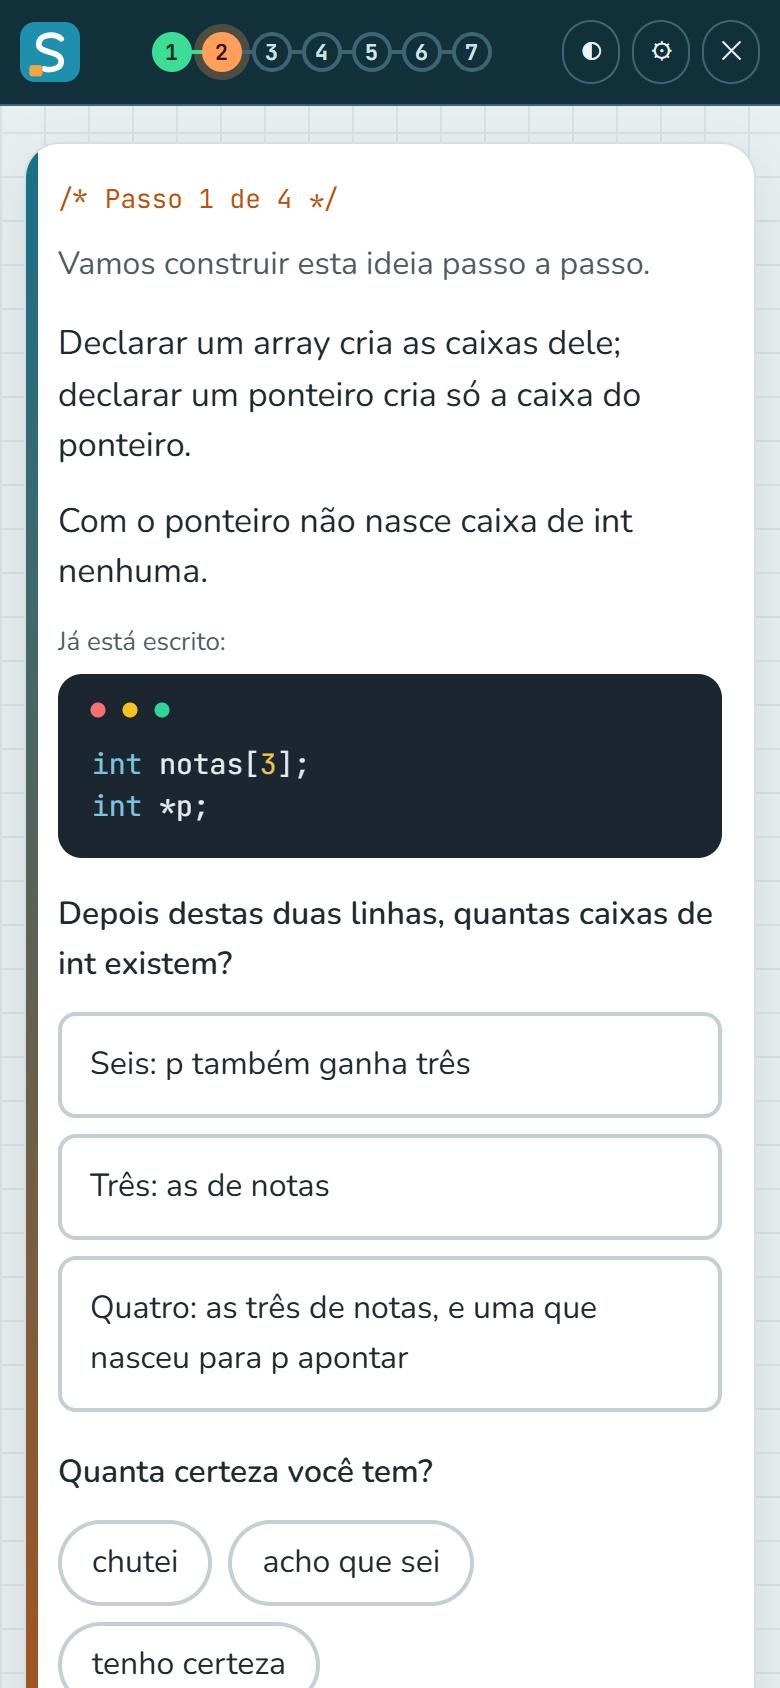
\includegraphics[width=.5\textwidth,height=.55\textheight,keepaspectratio]{fig-3-2-passo.jpg}
\fonte{Captura de tela do Structura, elaborada pelo autor.}
\end{figure}

Depois de todas as premissas, a reconferência faz uma pergunta para cada premissa trabalhada na sessão, ensinada ou corrigida, com outras premissas no meio. É o que separa ``acertou logo depois de ler'' de ``assimilou nesta sessão''. A pergunta é escolhida nesta ordem: o passo em que a pessoa tropeçou, na versão que ela não viu; um passo de produzir ainda não visto; uma questão do banco ainda não usada, que pergunta também a razão; e só então um passo já visto, com outros valores. Quando a razão marcada na reconferência é a concepção que tinha sido corrigida, o fechamento diz que ``a ideia voltou''.

O fechamento (Figura~\ref{fig:3-3}) resume a sessão em quatro blocos (as ideias erradas encontradas e se foram corrigidas; as lacunas, e em que passos; o que já estava firme; e o que ficou em aberto) e, abaixo, mostra a lista de premissas com o resultado de cada uma e o acesso à explicação. O passo em que a pessoa tropeçou aparece pelo nome dele, uma frase curta com a ideia do passo, e não pelo enunciado do exercício.

\begin{figure}[htbp]
\centering
\caption{O fechamento: as ideias erradas encontradas e a situação de cada uma}\label{fig:3-3}
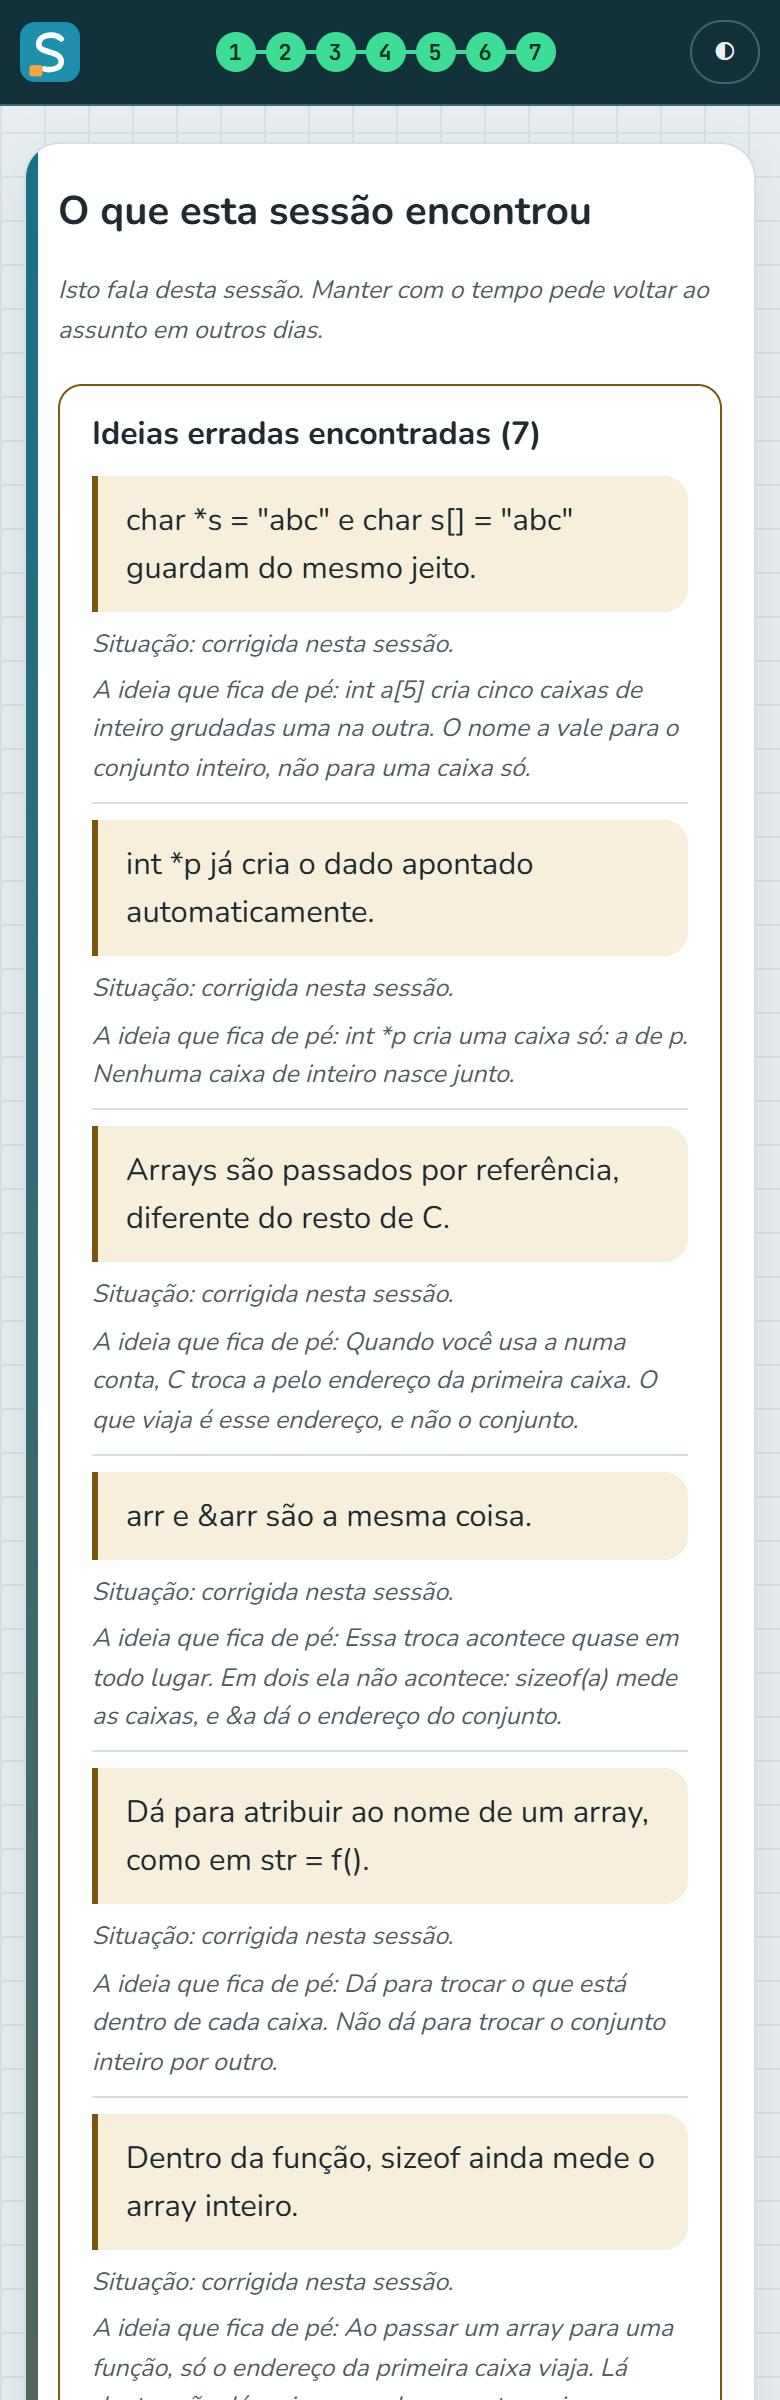
\includegraphics[width=.5\textwidth,height=.55\textheight,keepaspectratio]{fig-3-3-fechamento.jpg}
\fonte{Captura de tela do Structura, elaborada pelo autor.}
\end{figure}

\section{A escada de passos}

Cada premissa tem uma escada: uma sequência ordenada de passos, do mais mecânico até a ideia. Os passos guiados trazem uma ou duas frases curtas e um exercício pequeno; os de prática trazem só o exercício. A mesma escada serve para ensinar (a subida de quem não sabe), para treinar (depois da demonstração) e para reconferir (no fim).

Os exercícios têm cinco formas: tocar a parte de uma linha de código, montar uma linha a partir de peças, escolher entre alternativas, completar a lacuna de uma linha, e digitar a saída de um trecho. Cada passo tem duas versões (a segunda, com outros valores, é a que a reconferência usa), e todo erro previsto tem retorno próprio, que diz o que faltou e mostra o certo. As 79 premissas somam 402 passos (244 guiados e 158 de prática) e 804 versões. As formas se distribuem como no Quadro~\ref{qua:3-3}.

\begin{quadro}[htbp]
\caption{Os passos, por forma}\label{qua:3-3}
\footnotesize
\begin{tabularx}{\textwidth}{|X|l|}
\hline
\textbf{Forma} & \textbf{Passos} \\ \hline
escolher & 190 \\ \hline
digitar & 140 \\ \hline
montar & 37 \\ \hline
completar & 30 \\ \hline
tocar & 5 \\ \hline
\end{tabularx}
\fonte{Elaborado pelo autor.}
\end{quadro}

O texto de cada passo segue uma régua escrita, contra a qual o conteúdo foi revisado: um passo, uma ideia, com no máximo duas frases curtas antes do exercício; só usa o que um passo anterior já ensinou, neste tópico ou num anterior; primeiro o que se faz, depois a ideia; código que um iniciante escreveria; cada passo muda uma coisa só em relação ao anterior; e a analogia, quando há, vem depois do passo, nunca no lugar dele. Cada tópico trabalha as mesmas duas ou três variáveis do começo ao fim (no kc\_10, por exemplo, \texttt{idade} guarda um número, \texttt{p} o endereço de \texttt{idade} e \texttt{pp} o endereço de \texttt{p}), de modo que a declaração cresce e o cenário não muda.

\section{A demonstração com previsão}

Para cada concepção errônea de cada tópico há uma demonstração: um programa curto, de no máximo nove linhas, escrito com os nomes do cenário do tópico, e uma pergunta de previsão com duas alternativas: a que a máquina confirma e a que a concepção errônea espera (Figuras~\ref{fig:3-4}a e~\ref{fig:3-4}b). A pessoa prevê; depois vê o que aconteceu, e uma frase diz o que aquilo mostra e qual premissa fica de pé. As 61 concepções do catálogo dão 80 demonstrações porque 14 delas aparecem em mais de um tópico (a de que o ponteiro é o próprio dado, por exemplo, em quatro), e cada tópico tem a sua, com o cenário dele.

\begin{figure}[htbp]
\centering
\caption{(a) ``Você disse'': a concepção da pessoa e a previsão pedida; (b) ``A máquina respondeu'': o que o compilador disse, a previsão, e a ideia que fica de pé}\label{fig:3-4}
\begin{minipage}[t]{.48\textwidth}\centering
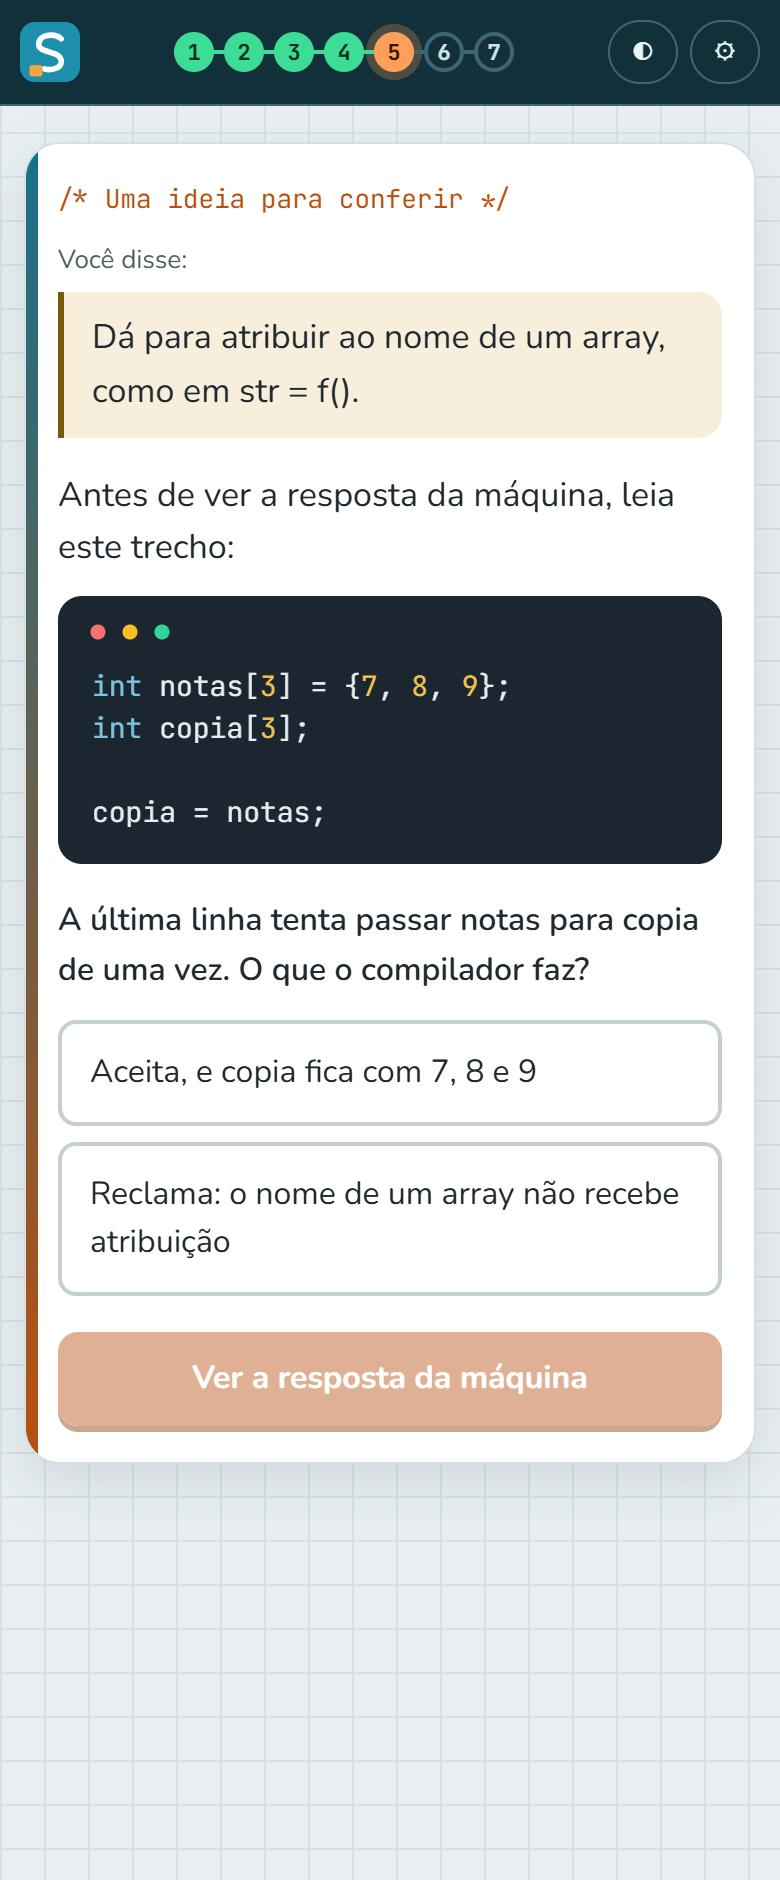
\includegraphics[width=\textwidth,height=.5\textheight,keepaspectratio]{fig-3-4a-voce-disse.jpg}\\[2pt]
(a)
\end{minipage}\hfill
\begin{minipage}[t]{.48\textwidth}\centering
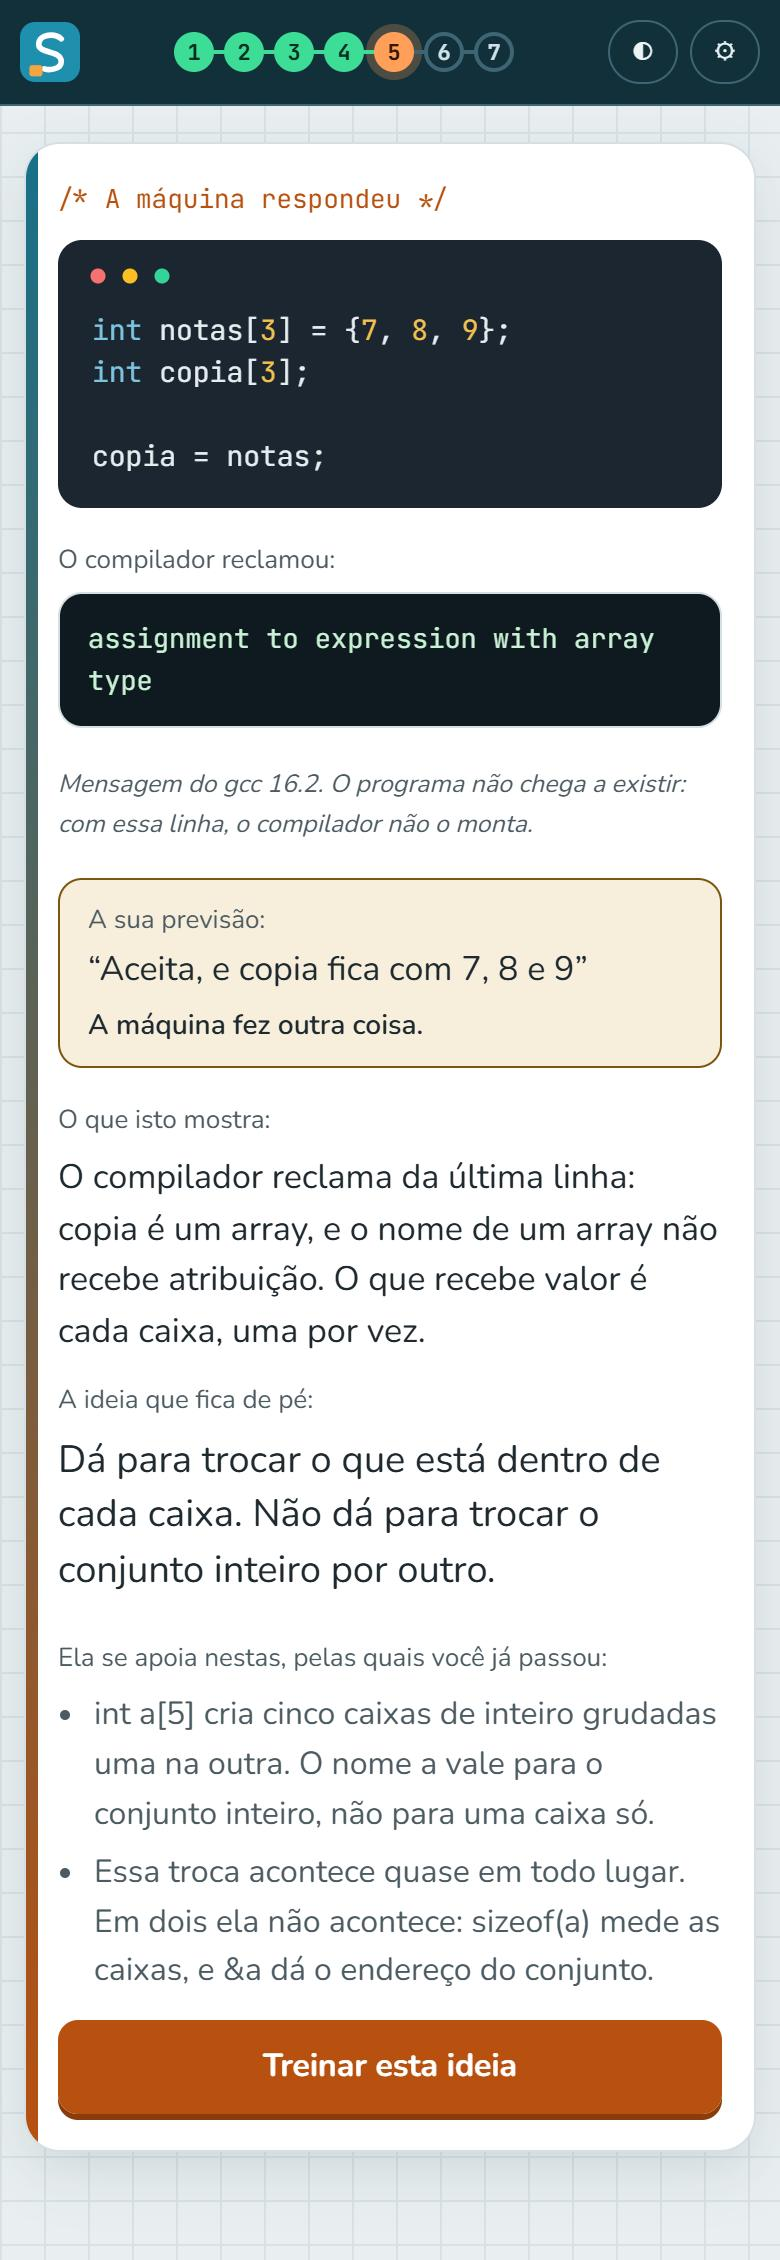
\includegraphics[width=\textwidth,height=.5\textheight,keepaspectratio]{fig-3-4b-maquina.jpg}\\[2pt]
(b)
\end{minipage}
\fonte{Captura de tela do Structura, elaborada pelo autor.}
\end{figure}

O que a máquina ``respondeu'' é de dois tipos. Em 41 das 80 demonstrações é a saída do programa: no kc\_11, por exemplo, quem acredita que a aritmética de ponteiros conta bytes prevê lixo para \texttt{*(p + 3)} sem \texttt{sizeof}, e vê sair o valor de \texttt{notas[3]}. Nas outras 39 é o que o compilador diz do programa: no kc\_12, quem acredita que \texttt{static} muda o escopo de uma variável prevê que o nome \texttt{n} passe a valer fora da função, e vê o compilador reclamar que \texttt{n} não foi declarado ali. Algumas dessas mensagens só aparecem com uma opção a mais do compilador (o analisador de fluxo, \texttt{-{}fanalyzer}, por exemplo, que aponta o bloco de memória pedido e nunca devolvido), e as opções permitidas formam uma lista fechada.

Quando o resultado depende do ambiente (o número de um endereço de memória, o tamanho de um tipo, o comportamento particular de um compilador), a demonstração traz uma nota de ambiente que diz isso com todas as letras. No kc\_12, o gcc 16.2 devolve \texttt{NULL} no lugar do endereço de uma variável local que deixou de existir; a demonstração que usa esse fato diz que é uma escolha do gcc, e que o padrão da linguagem não define aquele valor.

Toda demonstração foi conferida por compilador antes de entrar no sistema: a saída tem de ser a que o texto afirma, e a mensagem tem de sair de uma linha só, porque a tela diz ``o compilador reclamou desta linha'', e a mesma mensagem saindo de duas seria a demonstração dizer menos do que aconteceu. O Capítulo 5 descreve essa conferência.

\section{A cena}

A revisão de cada premissa tem uma cena: o trecho de código dela animado linha a linha (Figura~\ref{fig:3-5}). A linha que roda fica marcada no código, e um palco ao lado mostra o que ela fez: a caixa que nasce, o valor que entra e o que sai, o ponteiro com o seu bilhete, o que vai para a tela. São 79 cenas, uma por premissa.

\begin{figure}[htbp]
\centering
\caption{A cena da revisão do kc\_06 B1, dentro da bancada de \texttt{zera}: a cópia \texttt{n} vira 0, e \texttt{idade} continua 15}\label{fig:3-5}
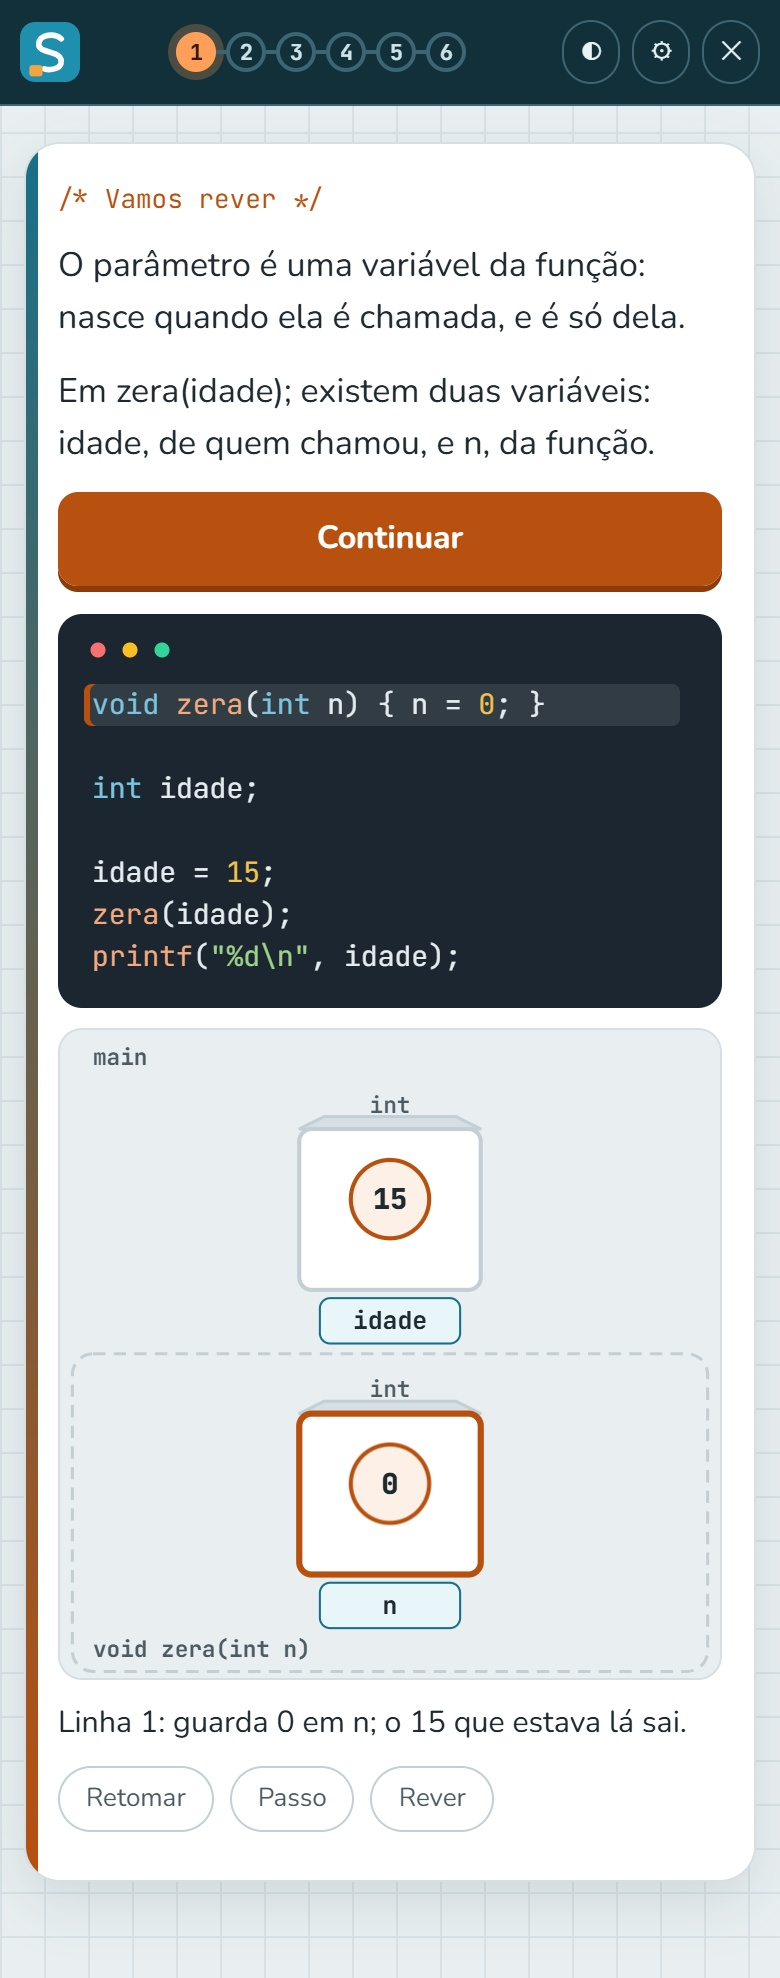
\includegraphics[width=.5\textwidth,height=.55\textheight,keepaspectratio]{fig-3-5-cena.jpg}
\fonte{Captura de tela do Structura, elaborada pelo autor.}
\end{figure}

Os personagens são poucos e vêm da mesma analogia em todos os tópicos. A caixa é a variável: uma etiqueta com o nome, o tipo escrito em cima e o valor numa bolinha dentro, com um ``?'' enquanto não há valor. O ponteiro é uma caixa que guarda um bilhete, ``→ idade'', com uma seta até a caixa apontada; o \texttt{NULL} é o bilhete que diz \texttt{NULL}, sem seta. A fileira é o array: as caixinhas lado a lado, com o índice embaixo, ou em linhas e colunas na matriz, e a caixinha que a linha lê ou escreve fica marcada; o texto entra como uma fileira de \texttt{char} com o \texttt{\textquotesingle{}\textbackslash{}0\textquotesingle{}} no fim. A bancada é a função enquanto roda: um andar próprio, com a primeira linha da função por título, onde nascem as caixas dela, que somem quando ela termina, menos a marcada \texttt{static}, que fica. E o bloco alugado é o que o \texttt{malloc} pede: ele mora num andar à parte, o monte, com a placa ``alugado'', e depois do \texttt{free} fica apagado, com a placa ``devolvido''.

A cena anda sozinha, um passo por segundo e pouco, com os botões Pausar, Passo e Rever. Quem pediu ao sistema operacional menos movimento vê a cena já no estado final, com o passo a passo nos botões. Cada passo tem uma frase, escrita embaixo do palco e lida pelos leitores de tela; por exemplo: ``Linha 3: guarda 21 em idade; o 20 que estava lá sai.'' Em tela de computador, a cena fica ao lado do texto da revisão; no celular, embaixo.

A cena é dado, e não desenho: cada uma é uma lista de passos, um por linha executada, com as ações daquela linha (criar uma caixa, guardar um valor, apontar, chamar e voltar de uma função, alugar e devolver um bloco). Por ser dado, ela é conferida contra o compilador como o resto do conteúdo (Capítulo 5): o palco nunca mostra um valor que o programa não tem.

\section{O registro e a retomada}

Tudo o que a pessoa faz é gravado num registro só de acréscimo, um evento por linha: a resposta, a razão, a certeza, o tempo, a previsão e se ela coincidiu com a concepção errônea, os passos errados, a reconferência. Nada é apagado ou reescrito. A sessão inteira pode ser reconstruída reexecutando as entradas gravadas: é assim que o sistema retoma uma sessão depois de o servidor reiniciar, e é por isso que tudo o que muda o caminho da sessão é entrada registrada. Como uma mudança nas regras faria as mesmas respostas caírem em telas diferentes, a primeira linha de cada sessão diz a versão das regras com que ela começou, e uma sessão de outra versão não é refeita: a pessoa vê uma mensagem, e não uma tela errada.

A identificação é por um código de participante, opcional e sem nenhum dado pessoal; o mesmo código retoma a sessão no mesmo tópico. Sem código, é o navegador que guarda o número da sessão: quem fecha a página e reabre o tópico volta à tela em que estava.

No meio da sessão, o botão Sair do topo oferece duas saídas. ``Guardar e sair'' volta à página dos tópicos, e a sessão continua de onde parou quando o tópico é reaberto. Não há o que gravar a mais, porque cada resposta já está no registro. ``Cancelar a sessão'', depois de uma confirmação, faz o tópico recomeçar do zero. Também o cancelamento não apaga nada: o registro ganha uma linha dizendo que a sessão foi cancelada, e daí em diante ela não é mais retomada: nem pelo número, nem pelo código, nem refeita depois de um reinício do servidor.

\section{A interface}

A interface foi desenhada para parecer um ambiente de programação, em dois temas: o escuro, inspirado num editor de código à noite (Figura~\ref{fig:3-6}), e o claro, com o topo escuro como a barra de um terminal (Figuras~\ref{fig:3-1} a~\ref{fig:3-4}). O tema é escolhido antes de a página ser desenhada (o do sistema operacional, ou o que a pessoa escolheu da última vez), e pode ser trocado por um botão no topo. Todos os pares de texto sobre fundo passam na razão de contraste de 4,5:1 que o critério 1.4.3 da WCAG 2.1, no nível AA, exige para texto comum \cite{w3c2025}, nos dois temas; quem pediu ao sistema operacional menos movimento não vê animação.

O código aparece numa moldura de editor, com cores por categoria (palavras-chave, números, textos, comentários, nomes de função); a saída do programa e a mensagem do compilador aparecem numa moldura de terminal, sem cores de código. O topo da trilha mostra o tópico e uma parada por premissa, numerada, com o estado de cada uma (feita, em aberto, agora ou ainda não), também dito em texto para leitores de tela, além dos botões de tema, de ajustes (o ritmo) e de sair. Em tela de celular os botões ficam só com o desenho, para que as oito paradas do kc\_09 caibam em 360 px de largura.

A página inicial desenha o caminho dos 13 tópicos como a trilha de um jogo (Figura~\ref{fig:3-6}): dez tópicos em fila, do kc\_00 ao kc\_09 (com o kc\_01, modelo de memória, depois do kc\_06 e do kc\_07), abrindo-se em três no fim (kc\_10, kc\_11 e kc\_12, que não dependem um do outro). A ordem é sugerida, e não imposta: todos os tópicos ficam abertos, e um teste confere que cada tópico vem depois dos seus pré-requisitos. Cada parada mostra o seu estado (já feito, próximo, em andamento ou aberto) e o andamento do tópico (``3 de 6''), e o próximo sugerido aparece num cartão acima do caminho.

\begin{figure}[htbp]
\centering
\caption{A página inicial no tema escuro: o próximo sugerido e o caminho dos 13 tópicos, com um tópico feito e um em andamento}\label{fig:3-6}
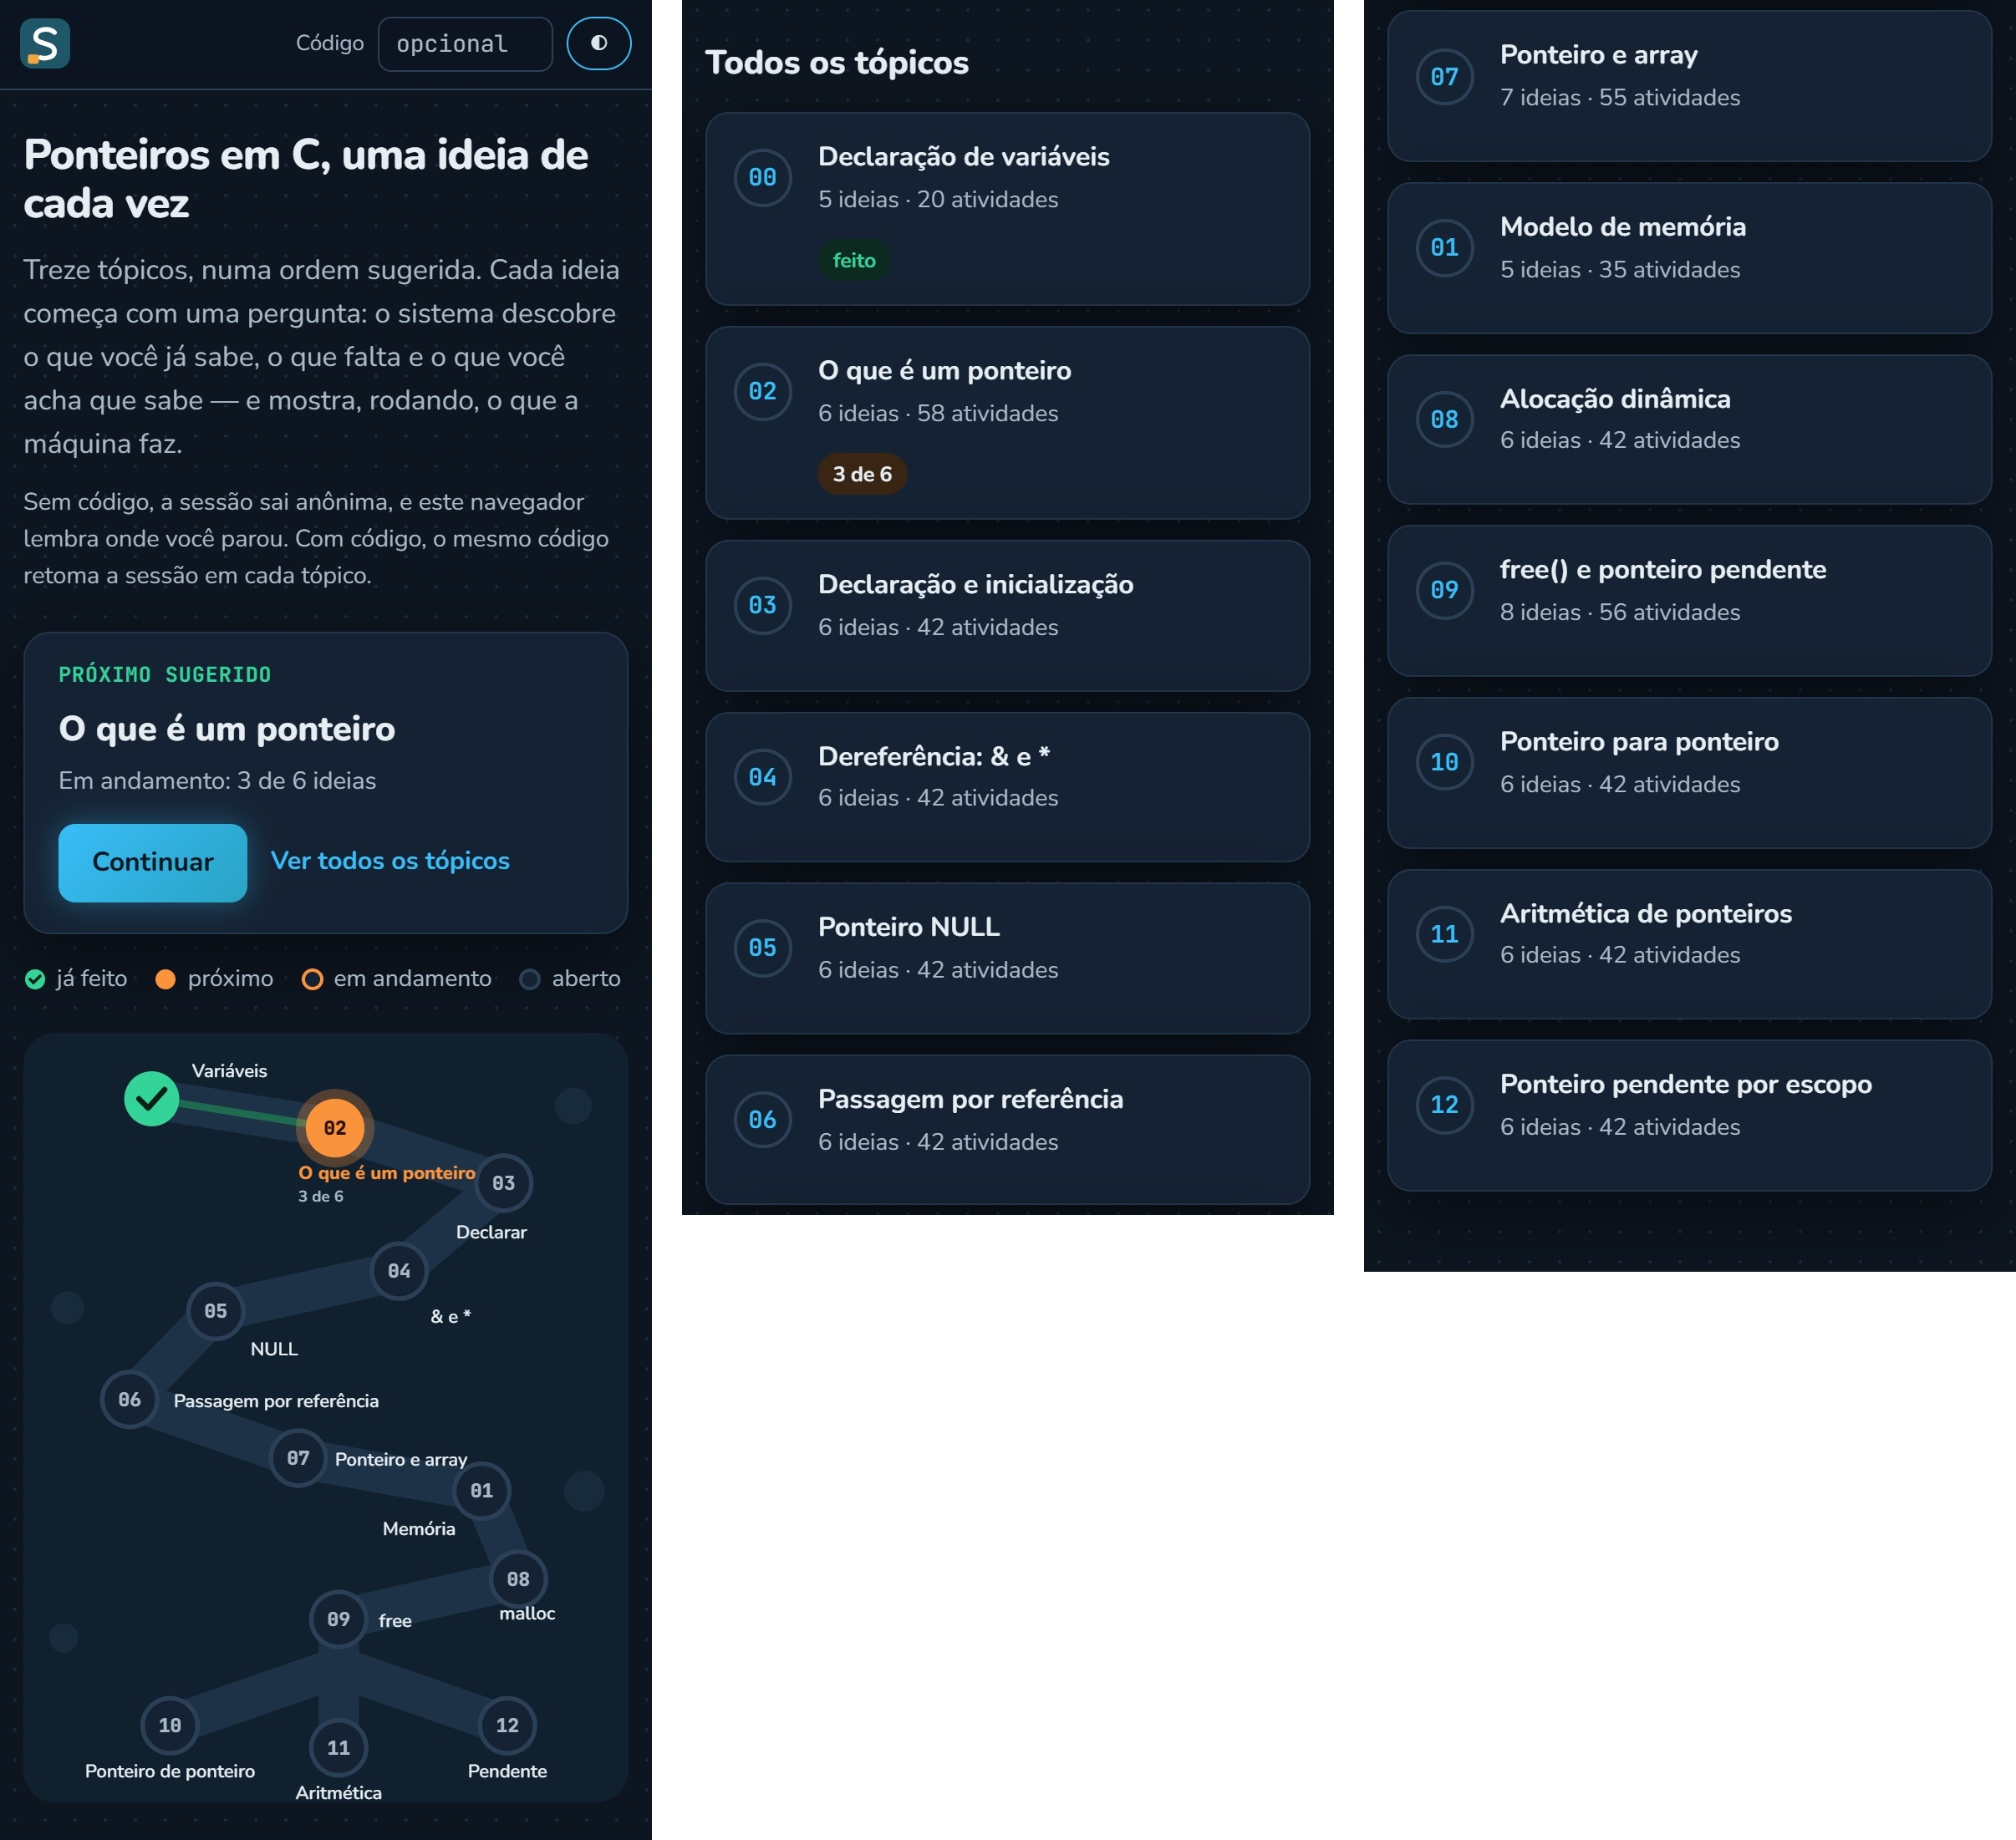
\includegraphics[width=.5\textwidth,height=.55\textheight,keepaspectratio]{fig-3-6-inicio-escuro.jpg}
\fonte{Captura de tela do Structura, elaborada pelo autor.}
\end{figure}

As fontes são livres (licença OFL) e estão guardadas no próprio projeto: nenhuma página carrega nada de outro endereço.

\section{Arquitetura}

O sistema é escrito em Python, com um servidor HTTP (FastAPI) e páginas em HTML, CSS e JavaScript sem dependências externas. O conteúdo (premissas, concepções errôneas, questões e escadas) fica em arquivos YAML, separados do código: acrescentar ou corrigir conteúdo não exige mexer no motor. O motor da trilha é uma função pura do estado da sessão e da entrada da pessoa, que devolve a próxima tela; é isso que torna a sessão reexecutável a partir do registro. Um portal monta os 13 tópicos num só servidor, que roda num contêiner Docker na própria máquina do laboratório, sem depender de serviço externo.
